\clearpage
\item \points{30} {\bf Incomplete, Positive-Only Labels}

In this problem we will consider training binary classifiers in situations
where we do not have full access to the labels. In particular, we consider
a scenario, which is not too infrequent in real life, where we have labels
only for a subset of the positive examples. All the negative examples and
the rest of the positive examples are unlabelled.

That is, we assume a dataset
$\{(x^{(i)}, t^{(i)}, y^{(i)} )\}_{i=1}^m$, where $t^{(i)}\in\{0, 1\}$ is
the ``true'' label, and where
\begin{equation*}
	y^{(i)} =
	\begin{cases} 
		1 & x^{(i)} \text{ is labeled} \\
		0 & \text{otherwise}. 
	\end{cases}
\end{equation*}
All labeled examples are positive, which is to say
$p(t^{(i)} = 1\mid y^{(i)} = 1) = 1$, but unlabeled examples may be positive or
negative. Our goal in the problem is to construct a binary classifier $h$ of
the true label $t$, with only access to the partial labels $y$. In other words,
we want to construct $h$ such that
 $h(x^{(i)}) \approx p(t^{(i)} = 1\mid x^{(i)})$ as closely as
possible, using only $x$ and $y$.

\emph{Real world example: Suppose we maintain a database of proteins which
are involved in transmitting signals across membranes. Every example added to
the database is involved in a signaling process, but there are many proteins
involved in cross-membrane signaling which are missing from the database.
It would be useful to train a classifier to identify proteins that
should be added to the database. In our notation, each example $x^{(i)}$
corresponds to a protein, $y^{(i)} = 1$ if the protein is in the database and
$0$ otherwise, and $t^{(i)} = 1$ if the protein is involved in a cross-membrane
signaling process and thus should be added to the database, and $0$ otherwise.}

\begin{enumerate}
	\item \subquestionpoints{5}
Suppose that each $y^{(i)}$ and $x^{(i)}$ are conditionally independent given
$t^{(i)}$:
%
\begin{equation*}
	p(y^{(i)} = 1\mid t^{(i)} = 1, x^{(i)}) = p(y^{(i)} = 1\mid t^{(i)} = 1).
\end{equation*}
%
Note this is equivalent to saying that labeled examples were selected uniformly
at random from the set of positive examples.
Prove that the probability of an example being labeled differs by a constant
factor from the probability of an example being positive. That is, show that
$p(t^{(i)} = 1\mid x^{(i)}) = p(y^{(i)} = 1\mid x^{(i)}) / \alpha$ for
some $\alpha\in\Re$.

\ifnum\solutions=1{
\begin{answer}
\begin{align*}
P(y=1|x) &= P(t=1|x) \cdot P(y=1|t=1,x)
    &= P(t=1|x) \cdot P(y=1|t=1)
\end{align*}
Obviously, $\alpha = P(y=1|t=1)$
\end{answer}

}\fi

	\clearpage
\item \subquestionpoints{5}
Suppose we want to estimate $\alpha$ using a trained classifier $h$ and a
held-out validation set $V$. Let $V_{+}$ be the set of labeled (and hence
positive) examples in $V$, given by $V_{+} = \{x^{(i)}\in V\mid y^{(i)} = 1\}$.
Assuming that  $h(x^{(i)})\approx p(y^{(i)} = 1\mid x^{(i)})$ for all
examples $x^{(i)}$, show that
%
\begin{equation*}
	h(x^{(i)}) \approx \alpha \quad\text{for all } x^{(i)}\in V_{+}.
\end{equation*}
%
You may assume that $p(t^{(i)} = 1\mid x^{(i)})\approx 1$ when
$x^{(i)}\in V_{+}$.

\ifnum\solutions=1 {
  \begin{answer}
We know the following equations:
\begin{align}
    h(x) &\approx P(y=1|x) = P(t=1|x) \cdot P(y=1|t=1)
    P(t=1|x) &= 1
\end{align}
So that, we can bring the second equation into the first equation.
\begin{align*}
    h(x) \approx 1 \cdot P(y=1|t=1) = \alpha
\end{align*}
\end{answer}

} \fi

	\clearpage
\item \subquestionpoints{5} \textbf{Coding problem.}
The following three problems will deal with a dataset which we have provided in
the following files:
%
\begin{center}
  \url{data/ds3_{train,valid,test}.csv}
\end{center}
%
Each file contains the following columns: $x_1$, $x_2$, $y$, and $t$. As in
Problem 1, there is one example per row.

First we will consider the ideal case, where we have access to the true
$t$-labels for training. In \texttt{src/p02cde\_posonly}, write a logistic
regression classifier that uses $x_1$ and $x_2$ as input features, and train it
using the $t$-labels (you can ignore the $y$-labels for this part). Output the
trained model's predictions on the test set to the file specified in the code.

\ifnum\solutions=1 {
  \begin{answer}
\end{answer}

} \fi

	\clearpage
\item \subquestionpoints{5} \textbf{Coding problem.}
We now consider the case where the $t$-labels are unavailable, so you only have
access to the $y$-labels at training time. Add to your code in
\texttt{p02cde\_posonly.py} to re-train the classifier (still using $x_1$ and
$x_2$ as input features), but using the $y$-labels only.

\ifnum\solutions=1 {
  \begin{answer}
\end{answer}

} \fi

	\clearpage
\item \subquestionpoints{10} \textbf{Coding problem.}
Using the validation set, estimate the constant $\alpha$ by averaging your
classifier's predictions over all labeled examples in the validation set:
%
\begin{equation*}
  \alpha \approx \frac{1}{|V_{+}|}\sum_{x^{(i)}\in V_{+}} h(x^{(i)}).
\end{equation*}
%
Add code in \texttt{src/p02cde\_posonly.py} to rescale your
classifier's predictions from part (d) using the estimated value for $\alpha$.

Finally, using a threshold of $p(t^{(i)} = 1 \mid x^{(i)}) = 0.5$, make three
separate plots with the decision boundaries from parts (c) - (e) plotted on top
of the test set. Plot $x_1$ on the horizontal axis and $x_2$ on the vertical
axis, and use two different symbols for the positive ($t^{(i)} = 1$) and
negative ($t^{(i)} = 0$) examples. In each plot, indicate the separating
hyperplane with a red line.

\ifnum\solutions=1 {
  \begin{answer}
\begin{figure}[h]
    \begin{subfigure}[b]{0.5\linewidth}
        \centering
        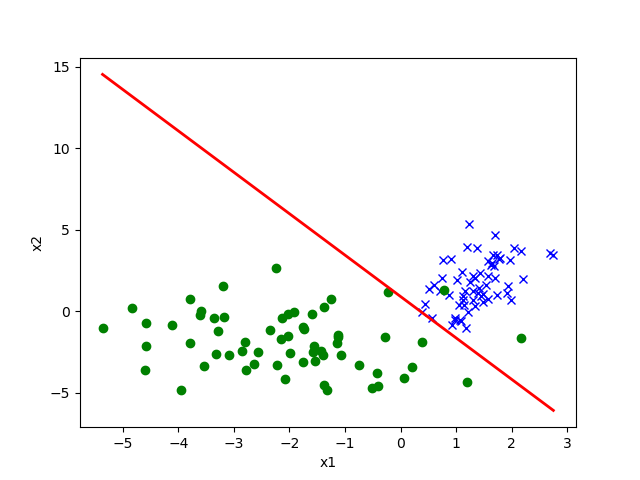
\includegraphics[width=\linewidth]{tex/p02c_pred.txt.png}
        \subcaption{2 c)}
    \end{subfigure}
    \begin{subfigure}[b]{0.5\linewidth}
        \centering
        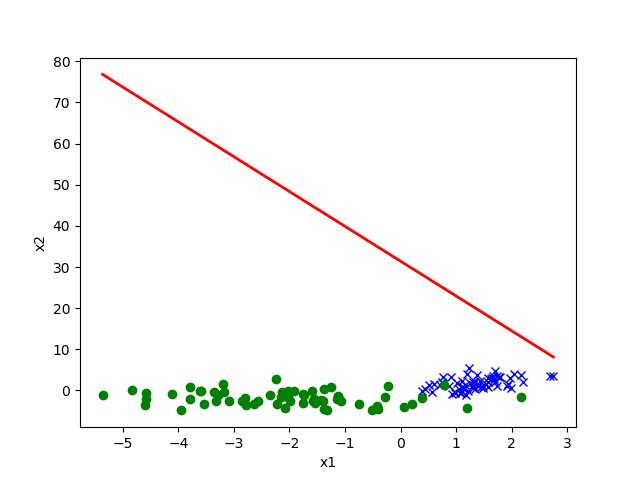
\includegraphics[width=\linewidth]{tex/p02d_pred.txt.png}
        \subcaption{2 d)}
    \end{subfigure}
    \begin{subfigure}[b]{0.5\linewidth}
        \centering
        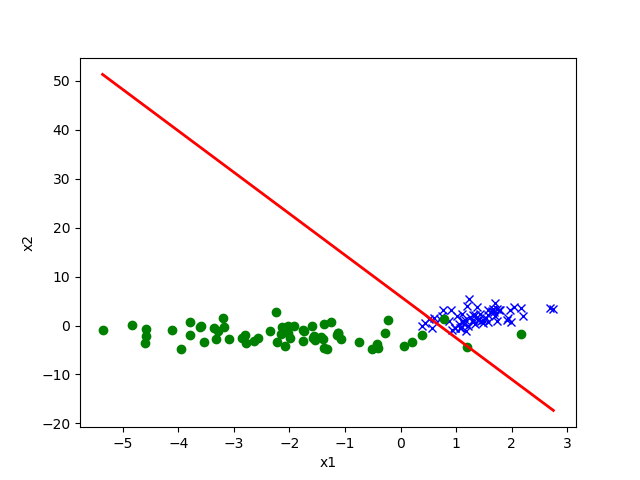
\includegraphics[width=\linewidth]{tex/p02e_pred.txt.png}
        \subcaption{2 e)}
    \end{subfigure}
\end{figure}
\end{answer}

} \fi

\end{enumerate}

\textbf{Remark}: We saw that the true probability $p(t\mid x)$ was only a
constant factor away from $p(y\mid x)$. This means, if our task is to only rank
examples (\emph{i.e.} sort them) in a particular order (e.g, sort the proteins
in order of being most likely to be involved in transmitting signals across
membranes), then in fact we do not even need to estimate $\alpha$. The rank
based on $p(y\mid x)$ will agree with the rank based on $p(t\mid x)$.
